% !TeX root = ../document.tex

\section{Results}

Within this section we will present the differences in the results of the aforementioned interpolation methods and different implementations. 

\begin{figure}
	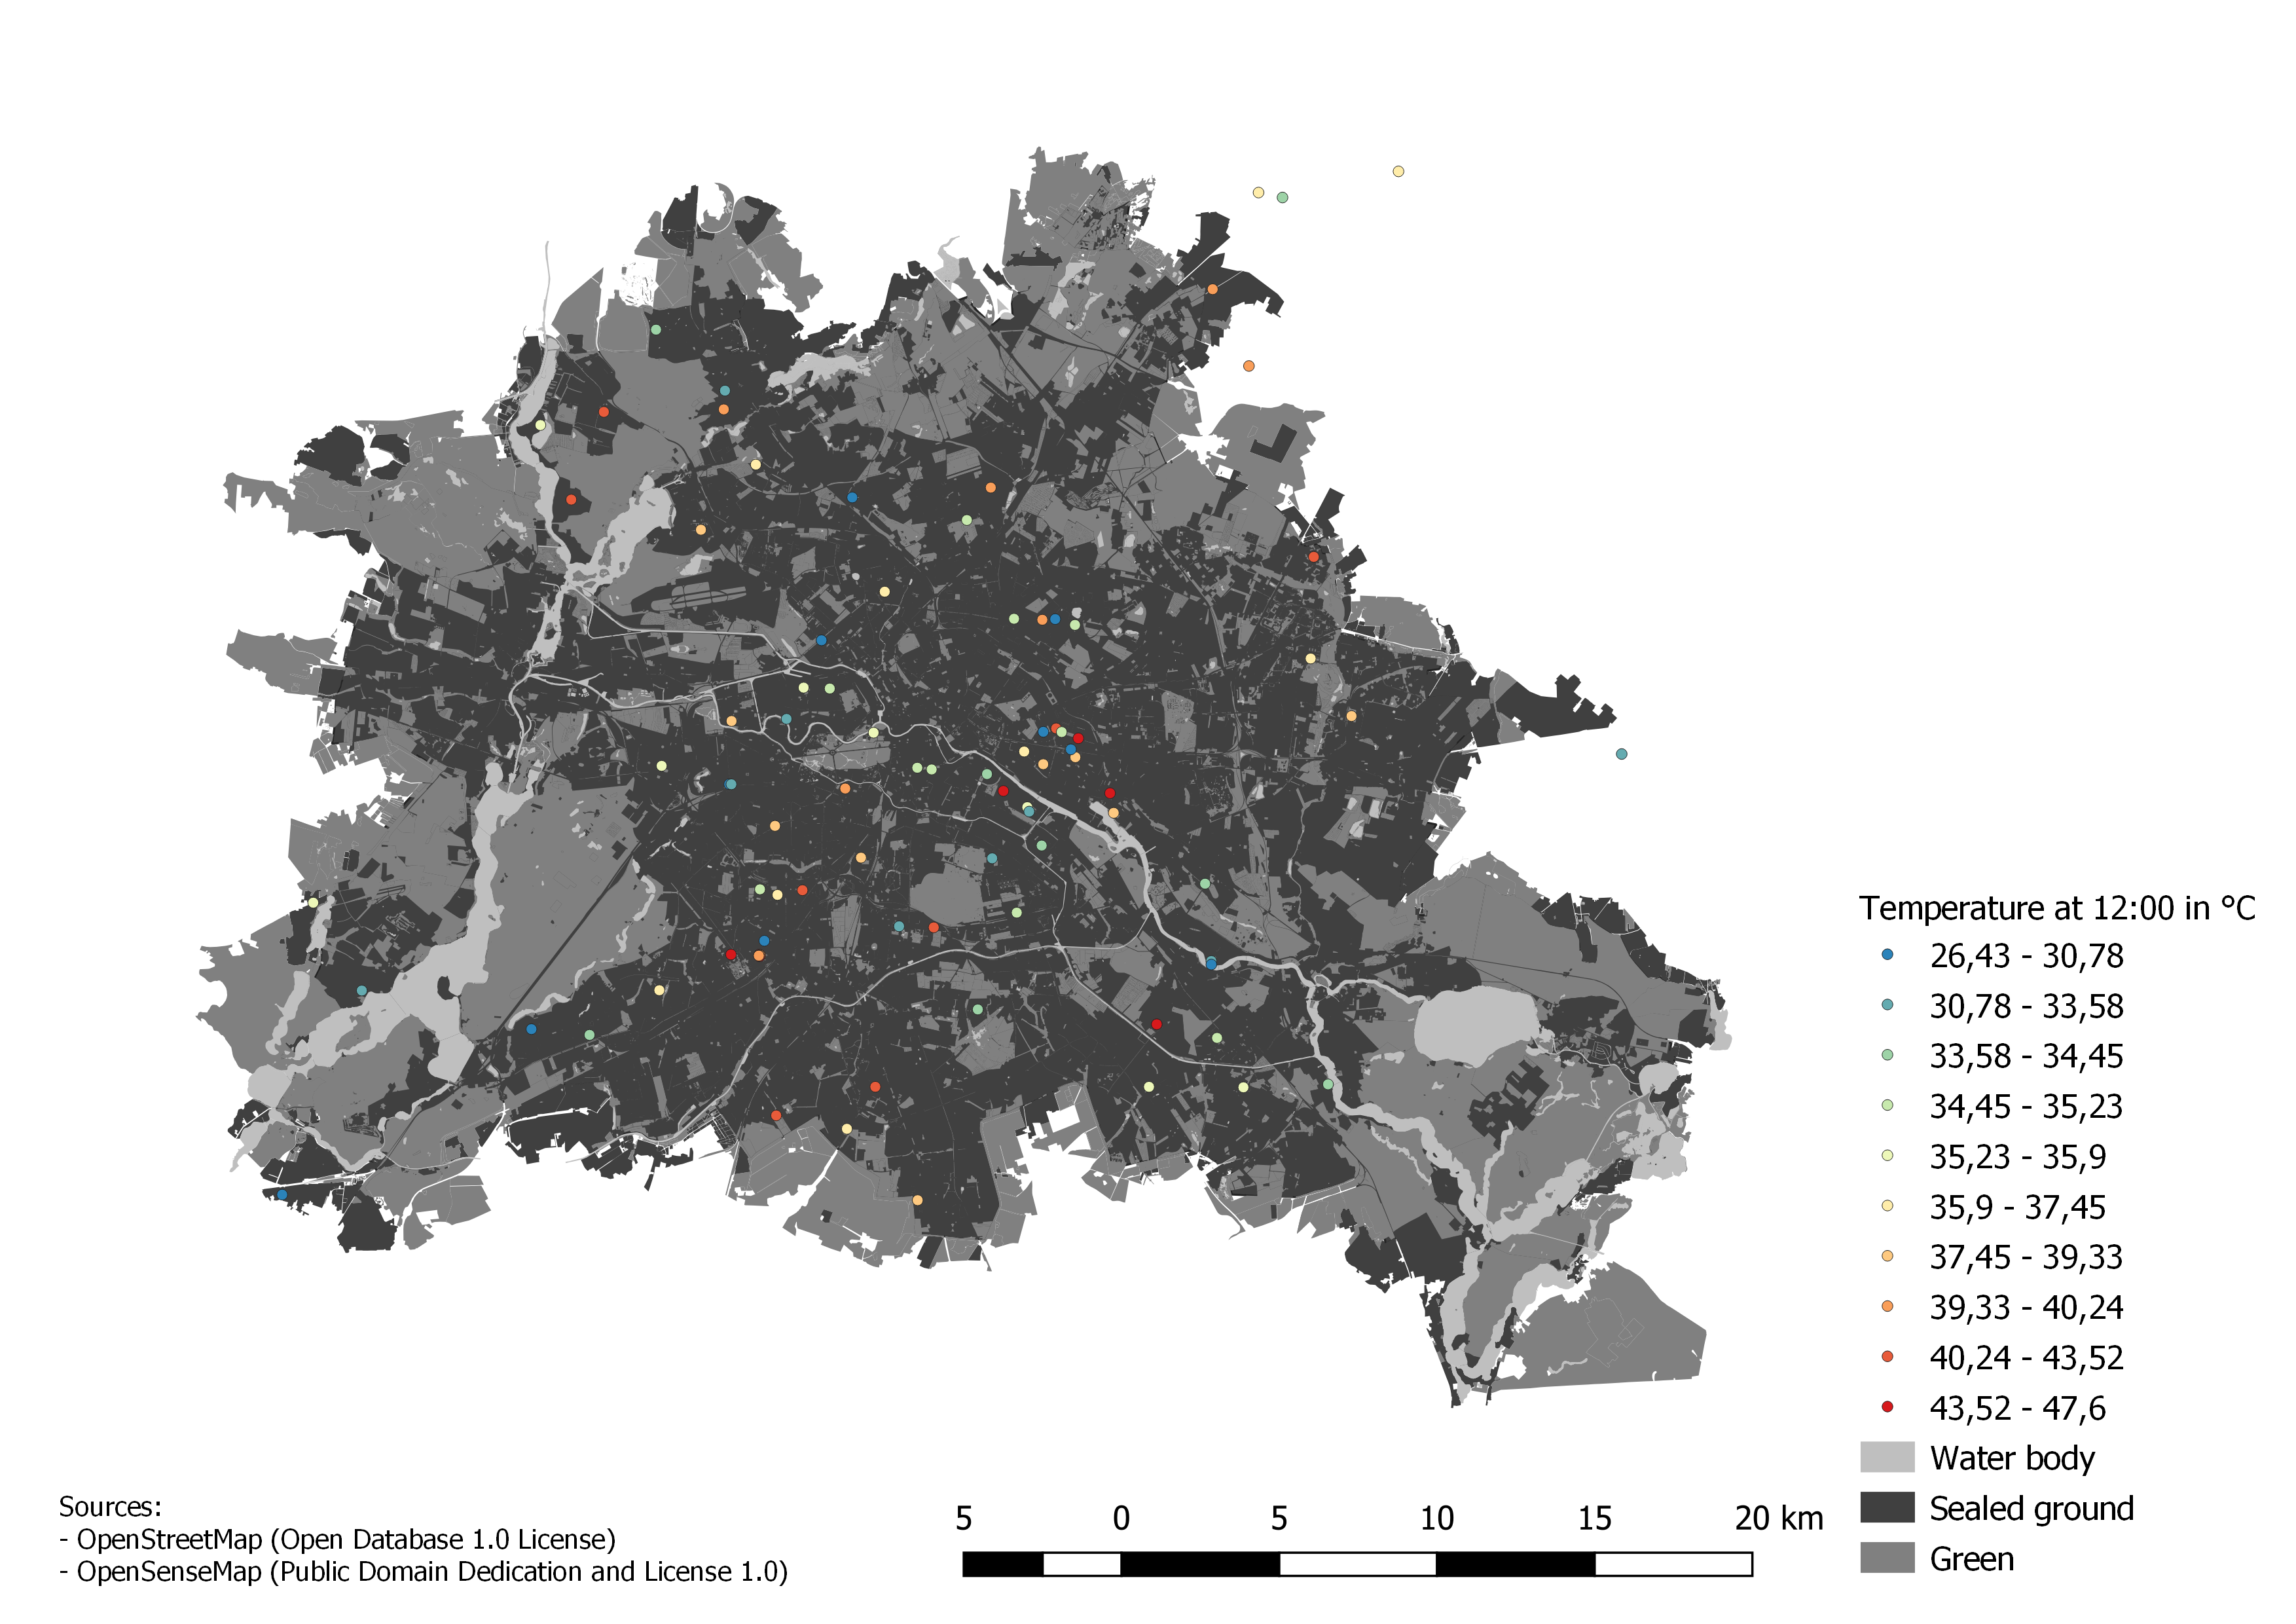
\includegraphics[width=\linewidth]{comparison/berlin.png}
	\caption{Surface types and sensor locations in research area}
	\label{fig:result_berlin}
\end{figure}

\subsection{Nearest neighbor}

The nearest neighbor interpolation (figure \ref{fig:result_nearest}) can easily be identified through sharp edges. The IUHI effect cannot be seen very clearly.

\begin{figure}
	\includegraphics[width=\linewidth]{images/interpolation_nearest.png}
	\caption{Nearest neighbor interpolation using GDAL}
	\label{fig:result_nearest}
\end{figure}

\subsection{TIN interpolation}

Figure \ref{fig:result_linear} shows the TIN interpolation as easily identified by the 

\begin{figure}
	\includegraphics[width=\linewidth]{images/interpolation_tin.png}
	\caption{TIN interpolation using GDAL}
	\label{fig:result_linear}
\end{figure}


\begin{figure}
	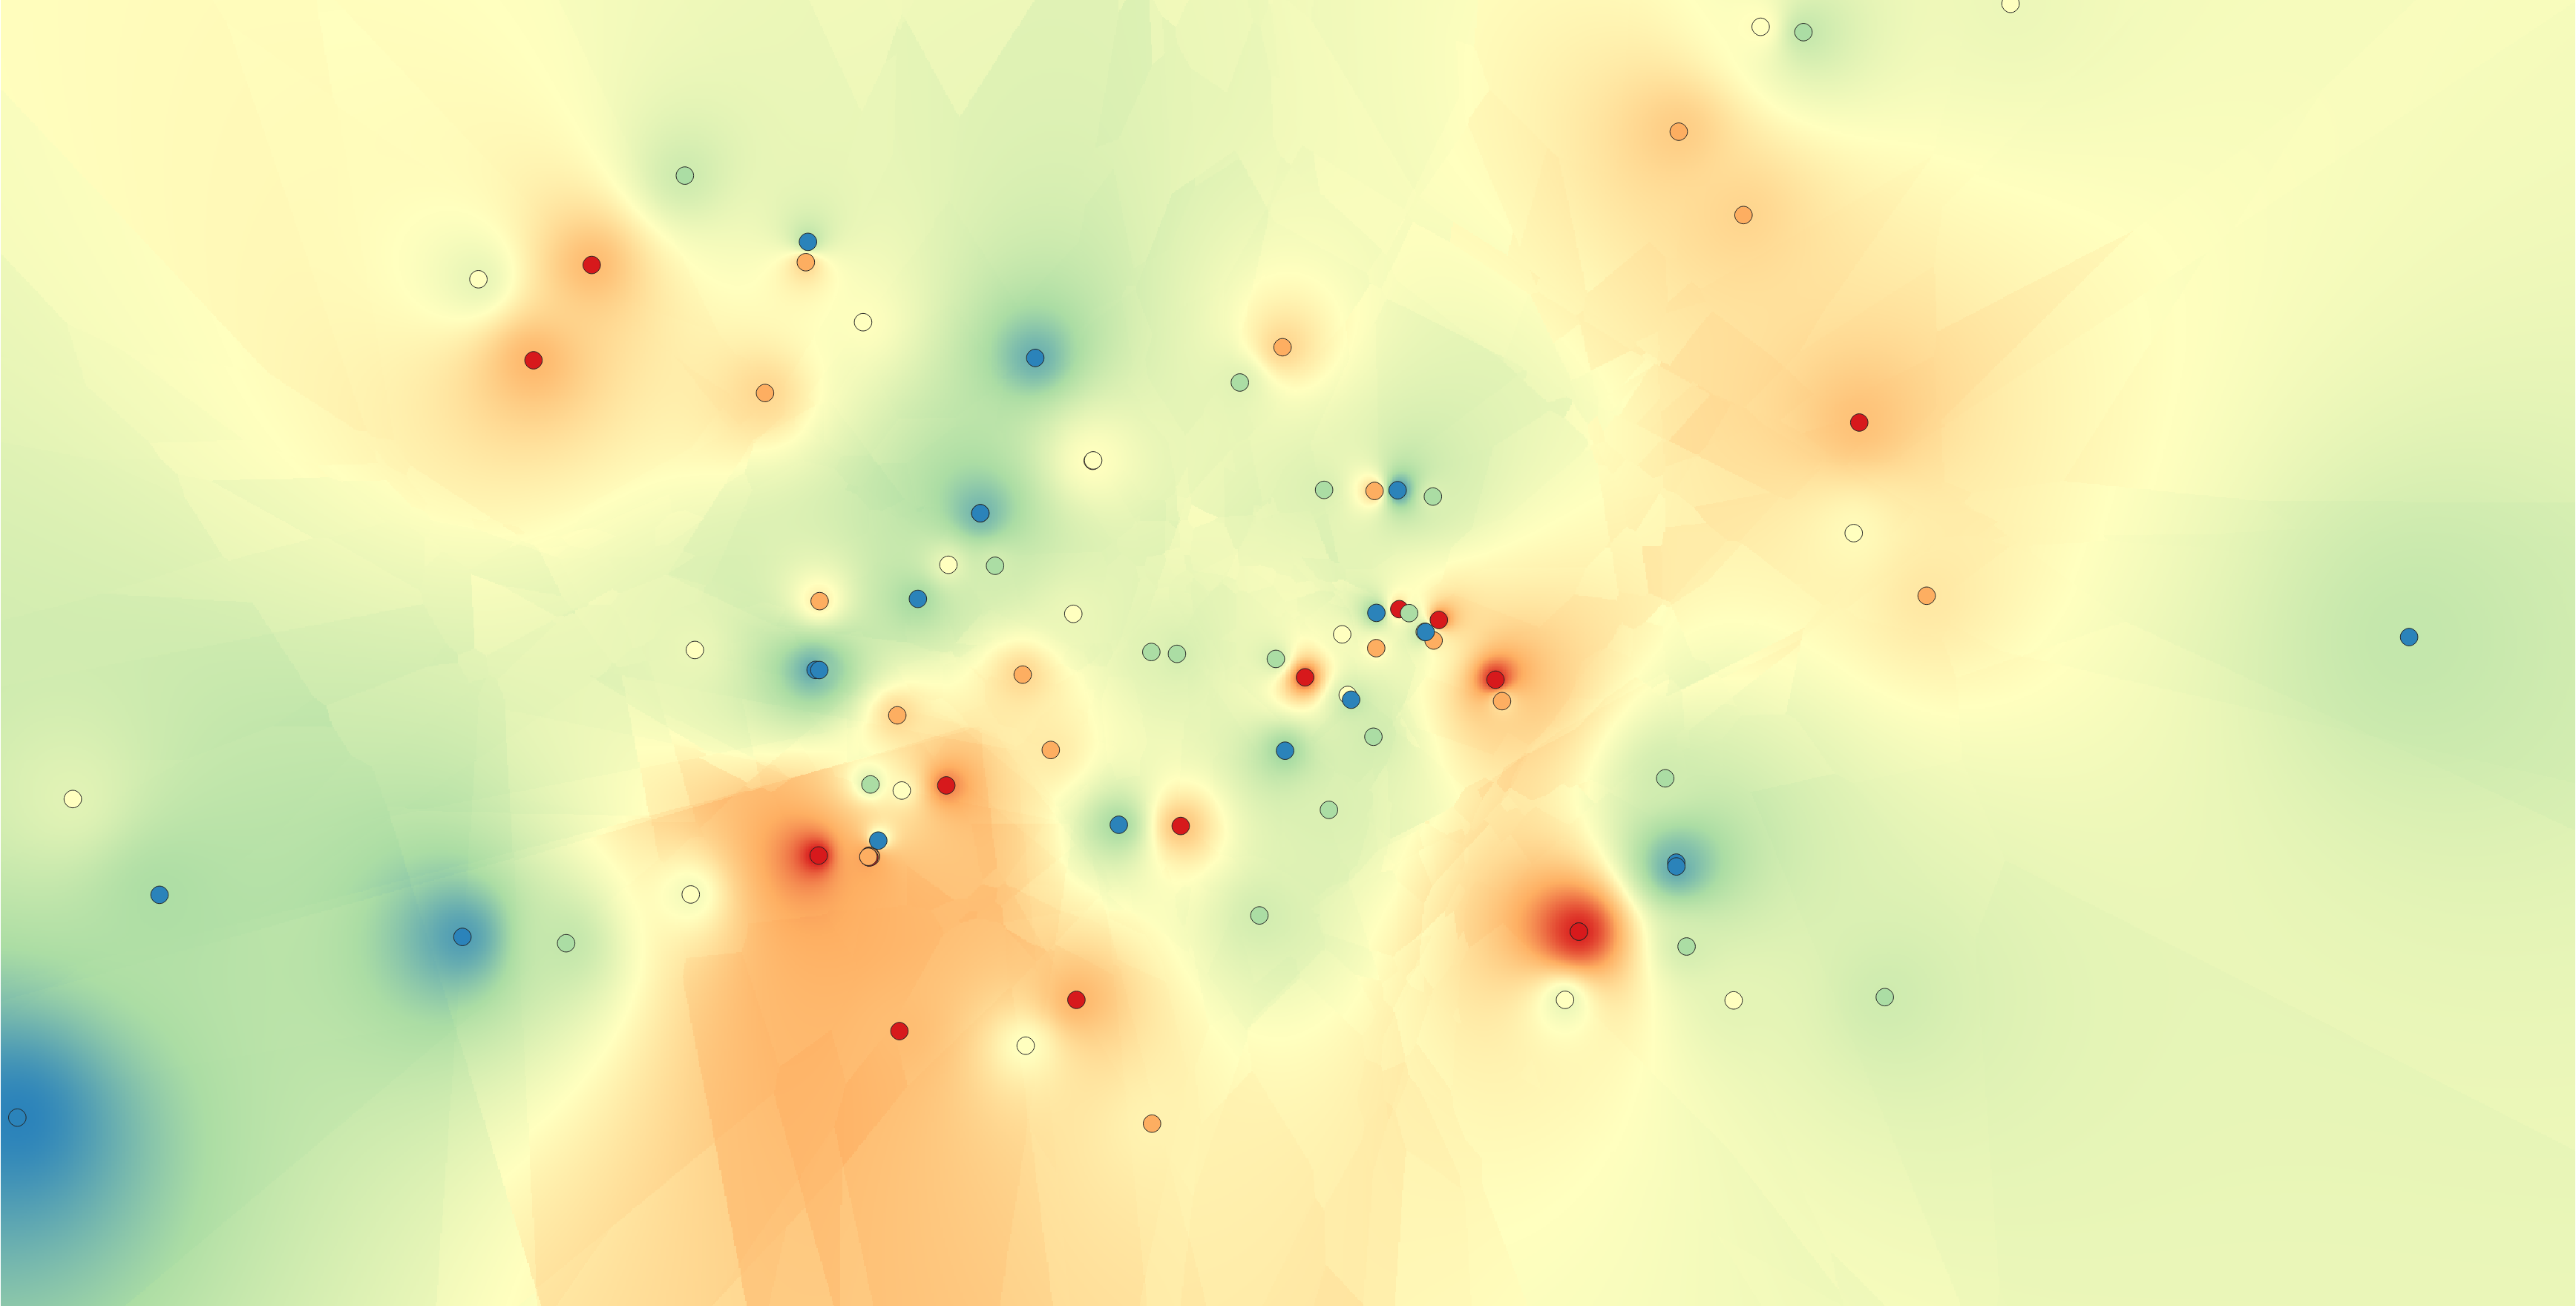
\includegraphics[width=\linewidth]{comparison/compare_idw_gdal.png}
	\caption{IDW interpolation using GDAL (12 max neighbors, power factor 2)}
	\label{fig:result_idw_gdal}
\end{figure}

\begin{figure}
	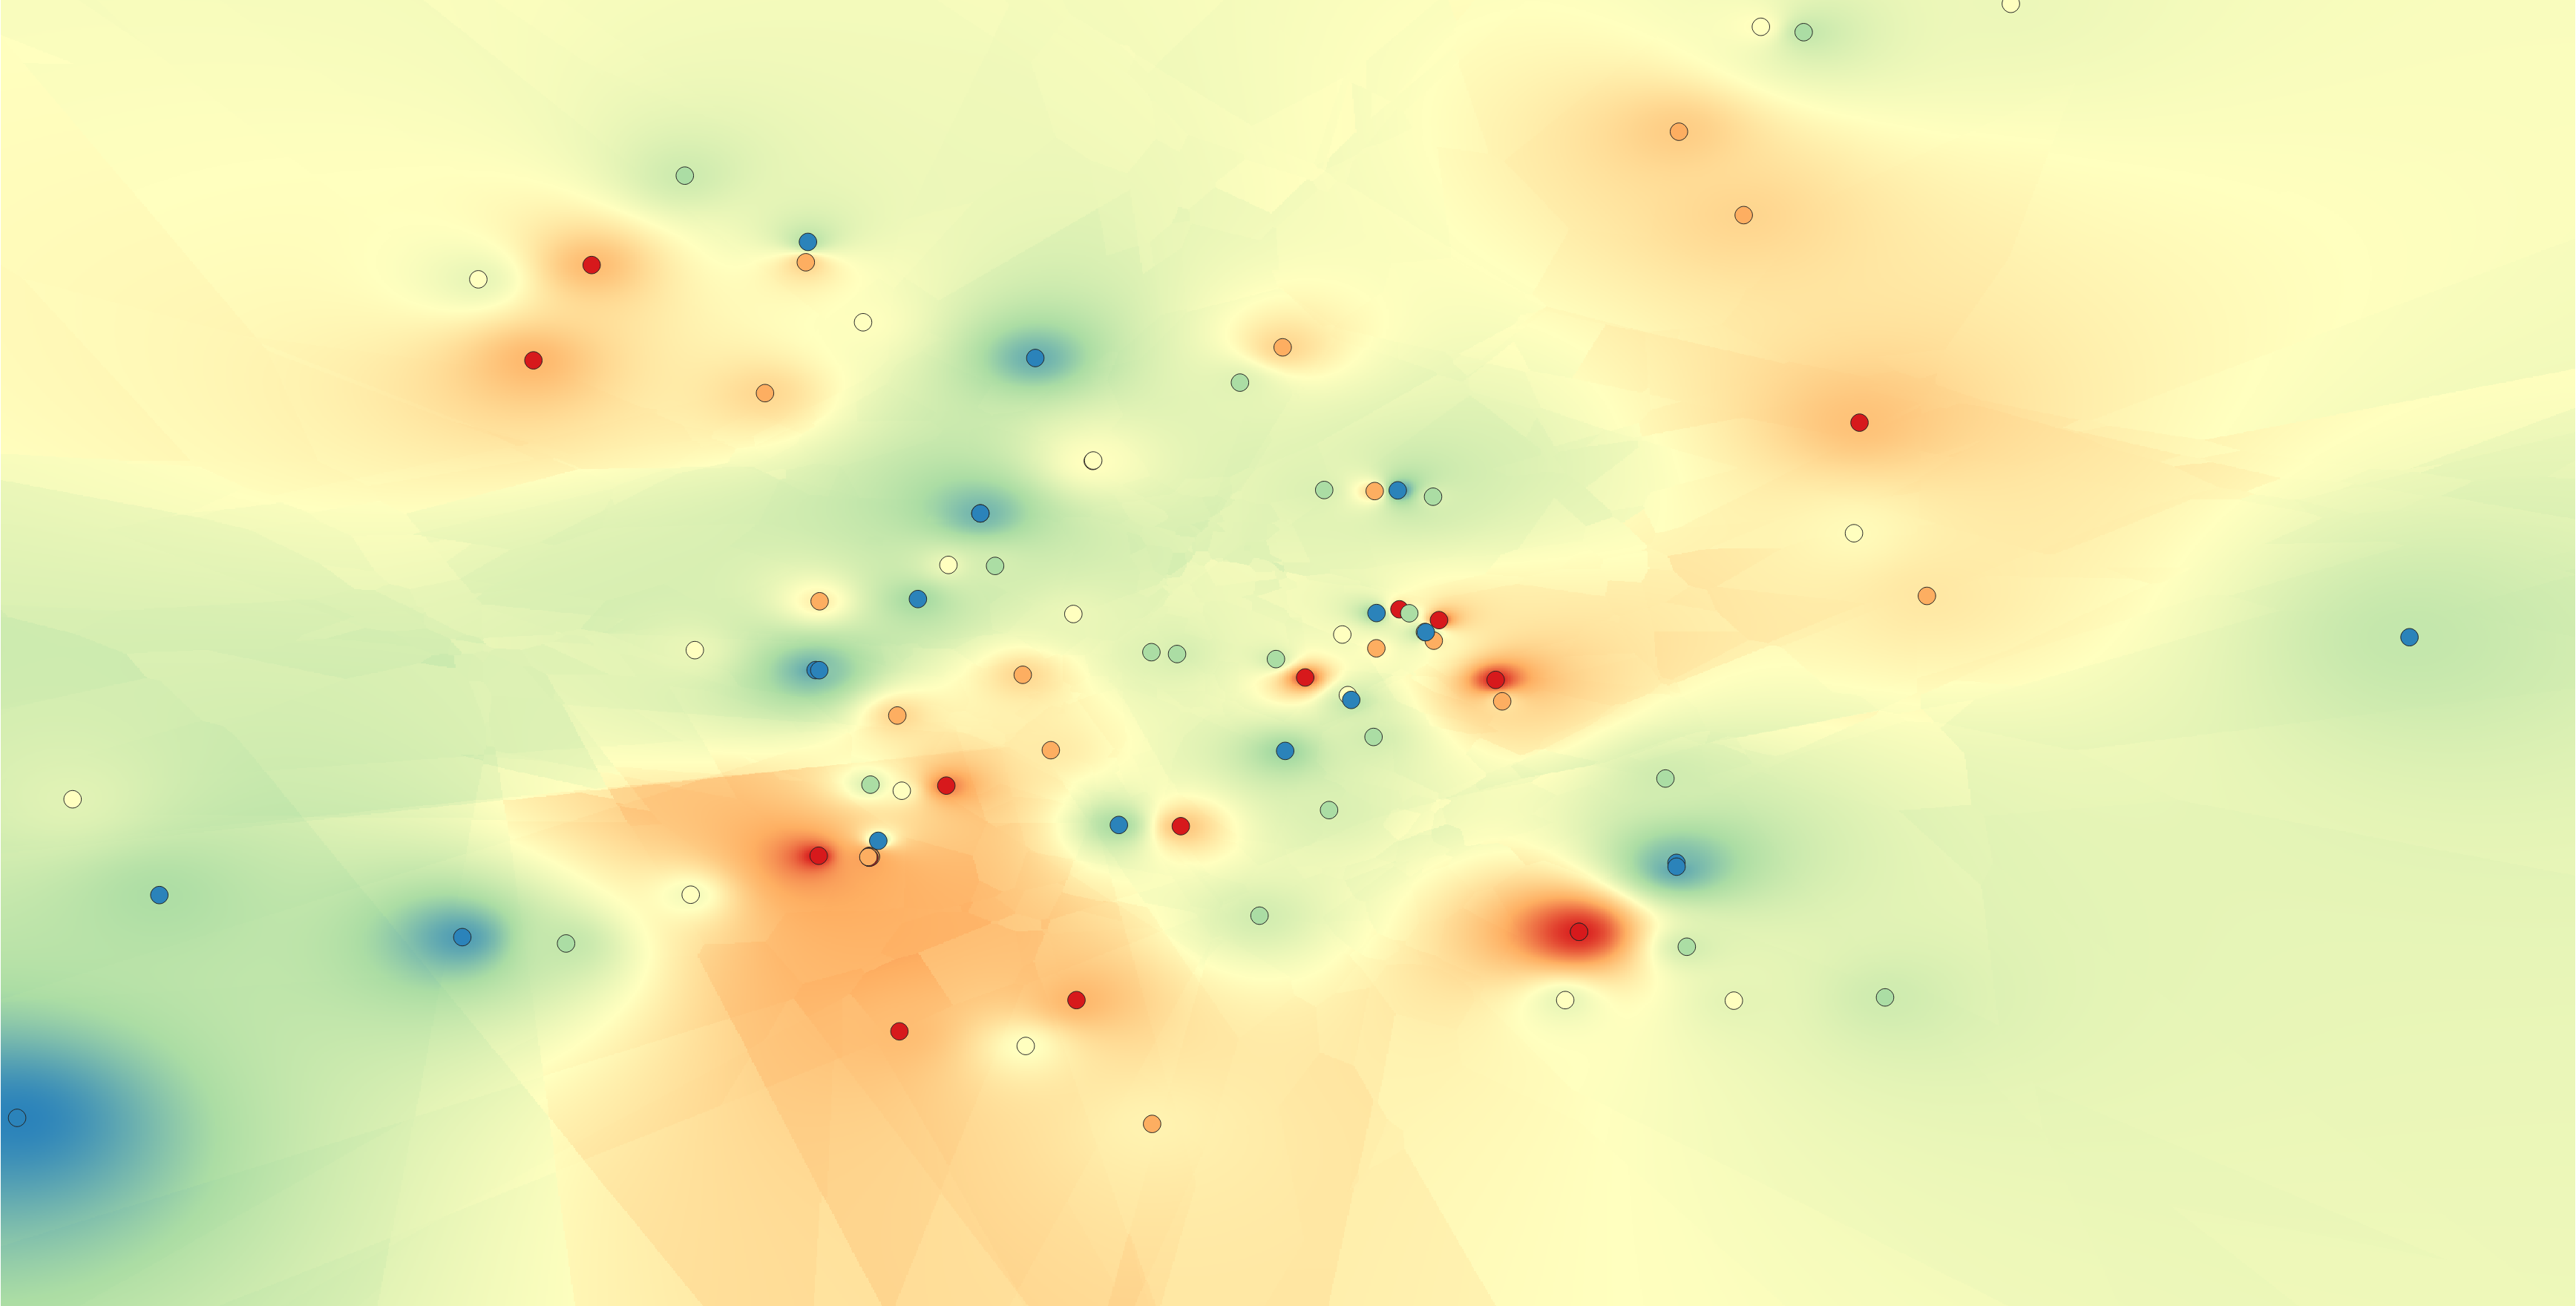
\includegraphics[width=\linewidth]{comparison/compare_idw_grass.png}
	\caption{IDW interpolation using GRASS GIS (12 max neighbors, power factor 2)}
	\label{fig:result_idw_grass}
\end{figure}

\begin{figure}
	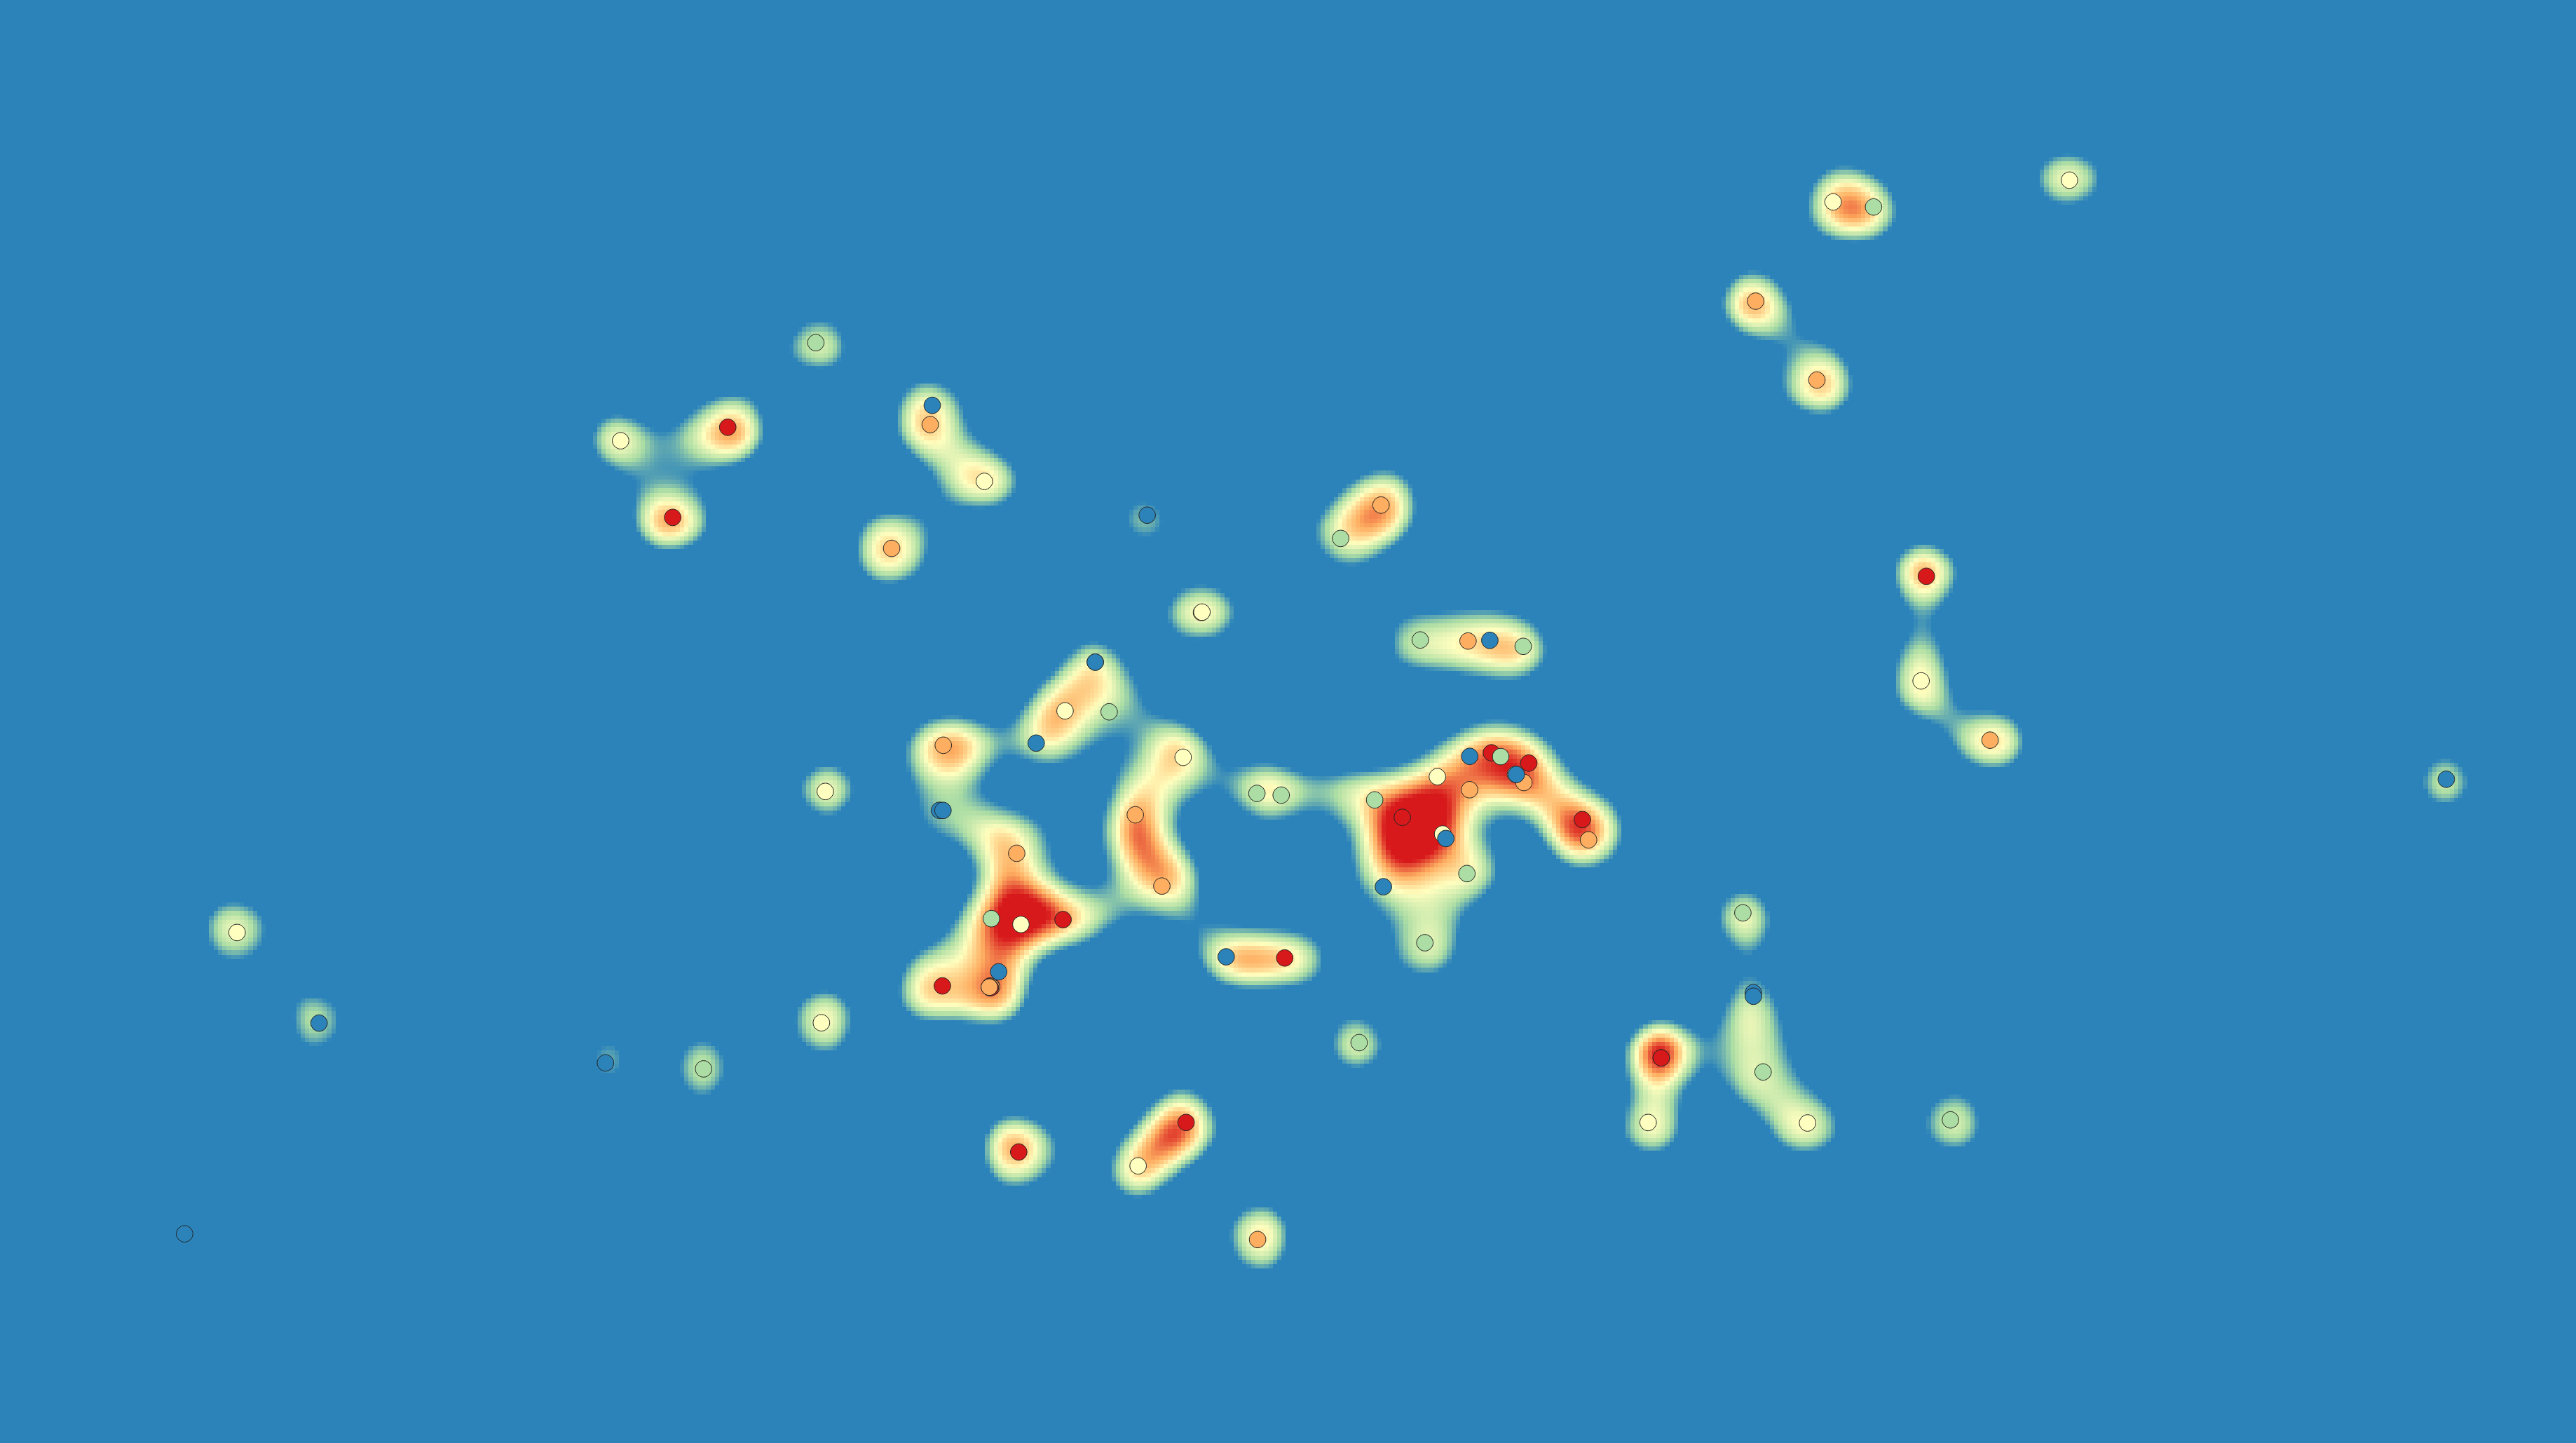
\includegraphics[width=\linewidth]{comparison/compare_bspline_saga.png}
	\caption{BSpline interpolation using GRASS GIS}
	\label{fig:result_bspline}
\end{figure}
